\documentclass[aspectratio=169]{../latex_main/tntbeamer}  % you can pass all options of the beamer class, e.g., 'handout' or 'aspectratio=43'
\usepackage{dsfont}
\usepackage{bm}
\usepackage[english]{babel}
\usepackage[T1]{fontenc}
%\usepackage[utf8]{inputenc}
\usepackage{graphicx}
\graphicspath{ {./figures/} }
\usepackage{algorithm}
\usepackage[ruled,vlined,algo2e,linesnumbered]{algorithm2e}
\usepackage{hyperref}
\usepackage{booktabs}
\usepackage{mathtools}

\usepackage{amsmath,amssymb}

\DeclareMathOperator*{\argmax}{arg\,max}
\DeclareMathOperator*{\argmin}{arg\,min}

\usepackage{amsbsy}
\newcommand{\vect}[1]{\bm{#1}}
%\newcommand{\vect}[1]{\boldsymbol{#1}}

\usepackage{pgfplots}
\pgfplotsset{compat=1.16}
\usepackage{tikz}
\usetikzlibrary{trees} 
\usetikzlibrary{shapes.geometric}
\usetikzlibrary{positioning,shapes,shadows,arrows,calc,mindmap}
\usetikzlibrary{positioning,fadings,through}
\usetikzlibrary{decorations.pathreplacing}
\usetikzlibrary{intersections}
\pgfdeclarelayer{background}
\pgfdeclarelayer{foreground}
\pgfsetlayers{background,main,foreground}
\tikzstyle{activity}=[rectangle, draw=black, rounded corners, text centered, text width=8em]
\tikzstyle{data}=[rectangle, draw=black, text centered, text width=8em]
\tikzstyle{myarrow}=[->, thick, draw=black]

% Define the layers to draw the diagram
\pgfdeclarelayer{background}
\pgfdeclarelayer{foreground}
\pgfsetlayers{background,main,foreground}

% Requires XeLaTeX or LuaLaTeX
%\usepackage{unicode-math}

\usepackage{fontspec}
%\setsansfont{Arial}
\setsansfont{RotisSansSerifStd}[ 
Path=../latex_main/fonts/,
Extension = .otf,
UprightFont = *-Regular,  % or *-Light
BoldFont = *-ExtraBold,  % or *-Bold
ItalicFont = *-Italic
]
\setmonofont{Cascadia Mono}[
Scale=0.8
]

\renewcommand{\ttdefault}{Cascadia Mono}

% scale factor adapted; mathrm font added (Benjamin Spitschan @TNT, 2021-06-01)
%\setmathfont[Scale=1.05]{Libertinus Math}
%\setmathrm[Scale=1.05]{Libertinus Math}

% other available math fonts are (not exhaustive)
% Latin Modern Math
% XITS Math
% Libertinus Math
% Asana Math
% Fira Math
% TeX Gyre Pagella Math
% TeX Gyre Bonum Math
% TeX Gyre Schola Math
% TeX Gyre Termes Math

% Literature References
\newcommand{\lit}[2]{\href{#2}{\footnotesize\color{black!60}[#1]}}

%%% Beamer Customization
%----------------------------------------------------------------------
% (Don't) Show sections in frame header. Options: 'sections', 'sections light', empty
\setbeamertemplate{headline}{empty}

% Add header logo for normal frames
\setheaderimage{
	% 
\includegraphics[height=\logoheight]{figures/TNT_darkv4.pdf}
	
\includegraphics[height=\logoheight]{../latex_main/figures/Leibniz-AI-Academy_Logo}
	% 
\includegraphics[height=\logoheight]{figures/logo_tntluh.pdf}
}

% Header logo for title page
\settitleheaderimage{
	% 
\includegraphics[height=\logoheight]{figures/TNT_darkv4.pdf}
	
\includegraphics[height=\logoheight]{../latex_main/figures/Leibniz-AI-Academy_Logo}
	% 
\includegraphics[height=\logoheight]{figures/logo_tntluh.pdf}
}

% Title page: tntdefault 
\setbeamertemplate{title page}[tntdefault]  % or luhstyle
% Add optional title image here
%\addtitlepageimagedefault{
\includegraphics[width=0.65\textwidth]{figures/luh_default_presentation_title_image.jpg}}

% Title page: luhstyle
% \setbeamertemplate{title page}[luhstyle]
% % Add optional title image here
% \addtitlepageimage{
\includegraphics[width=0.75\textwidth]{figures/luh_default_presentation_title_image.jpg}}

\author[Abedjan \& Lindauer]{Ziawasch Abedjan \& \underline{Marius Lindauer}\\[1em]
	%
\includegraphics[height=\logoheight]{../latex_main/figures/luh_logo_rgb_0_80_155.pdf}\qquad
	
\includegraphics[height=\logoheight]{../latex_main/figures/DBIS_Kurzlogo.png}\qquad

\includegraphics[height=\logoheight]{../latex_main/figures/logo_short_highres_black}\qquad

\includegraphics[height=\logoheight]{../latex_main/figures/Leibniz-AI-Academy_Logo}\qquad
%
\includegraphics[height=\logoheight]{../latex_main/figures/L3S.jpg}	
}
\date{\hspace{0.5em} {
\includegraphics[height=1.5em]{../latex_main/figures/Cc-by-nc-sa_icon.svg.png}}; extension of \href{https://ds100.org/fa21/}{[DS100]}
}


%%% Custom Packages
%----------------------------------------------------------------------
% Create dummy content
\usepackage{blindtext}

% Adds a frame with the current page layout. Just call \layout inside of a frame.
\usepackage{layout}


%%% Macros
%\renewcommand{\vec}[1]{\mathbf{#1}}
% \usepackage{bm}
%\let\vecb\bm

\title[Evaluation]{DS: Evaluation}
\subtitle{Assessment}

\graphicspath{ {./figure/} }
%\institute{}


\begin{document}
	
	\maketitle
	
	\begin{frame}{Generalization: Train-Validation-Test}
	       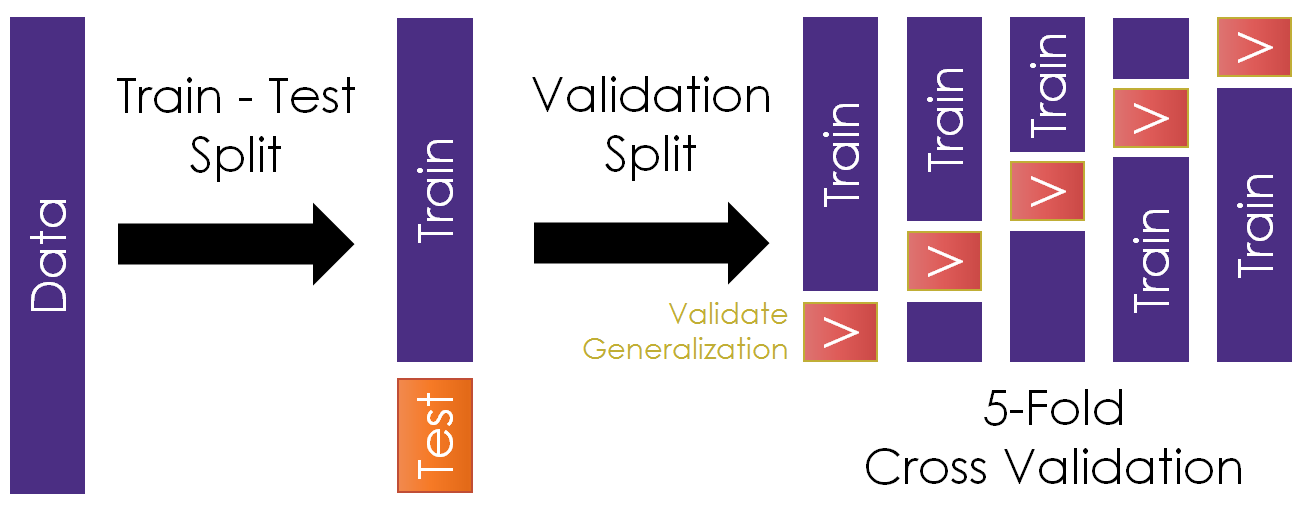
\includegraphics[scale=.43]{Bild4}\\
	\end{frame}
	
	\begin{frame}[c]{What to optimize for?}
	    \begin{itemize}
	        \item Let's stick to classification for the moment
                \medskip
                \item Metrics for learning your model on include
                    \begin{enumerate}
                        \item Cross entropy
                        \item Hinge loss
                    \end{enumerate}
                \item Would we use cross entropy to validate our model later on?
                \break
                \item[$\leadsto$] No!
                \begin{itemize}
                    \item Cross entropy (and other training loss metrics) has nice properties for training your model
                    \item But, eventually your application will tell you which metric we care about
                    \item For example, it could be accuracy
                    $$ \text{acc} = \frac{N_{\text{correct}}}{N_{\text{all}}} $$
                \end{itemize}
	    \end{itemize}
	\end{frame}

        \begin{frame}[c]{Best Practices}
	    \begin{enumerate}
	        \item \textbf{Understand the Business Objective:}
                \begin{itemize}
                    \item Your evaluation metric should align with the business or research objectives. For instance, in a fraud detection scenario, false negatives (a fraudulent transaction is marked as non-fraudulent) can be much more harmful than false positives (a non-fraudulent transaction is marked as fraudulent). So, even if your training loss is low, if your evaluation metric doesn't reflect the true cost of errors, your model may not be as effective as you think.
                \end{itemize}
                \pause
                \item \textbf{Differentiate between Training and Validation Metrics:}
                \begin{itemize}
                    \item Training losses are often designed to be easy to optimize, e.g., cross entropy
                    \item Your validation loss should be informative and interpretable; cross-entropy is often neither
                    \item Your validation metric should always be chosen to reflect the final objective of the model
                \end{itemize}
                \pause
                \item \textbf{Consider the Data Distribution}
                \begin{itemize}
                    \item If the dataset is imbalanced (i.e., not classes are represented equally in your dataset), metrics like accuracy might not be useful
                    \item For example, in a binary classification problem with 95\% instances belonging to Class 1, a dumb model predicting everything as Class 1 will still have 95% accuracy.
                \end{itemize}
	    \end{enumerate}

	\end{frame}

         \begin{frame}[c]{Best Practices (cont'd)}
	    \begin{enumerate}\setcounter{enumi}{3}
                \item \textbf{Take into Account the Type of Task}
                \begin{itemize}
                    \item Different tasks and learning paradigms require different metrics
                    \item For regression tasks, Mean Squared Error (MSE) or Mean Absolute Error (MAE) are common metrics
                    \item For classification tasks, accuracy, precision, recall, F1-score, or AUC-ROC might be used
                \end{itemize}
                \pause
                \item \textbf{Consistency of Metrics}
                \begin{itemize}
                    \item The training metric should ideally be similar to the evaluation metric
                    \item If they are not, it's essential to monitor both during the training phase
                    \item If the training metric improves but the evaluation metric does not, it's an indication that the model might be overfitting
                    \item Validation metric and test metric should always be the same!
                \end{itemize}
                \pause
                \item \textbf{Understand Trade-offs}
                \begin{itemize}
                    \item Realize that there's often a trade-off between different metrics, especially in classification problems
                    \item One metric might go up while another goes down
                    \item Understand these trade-offs and select a metric that aligns with your business or research objective
                \end{itemize}
	    \end{enumerate}

	\end{frame}

        \begin{frame}[c]{Best Practices (cont'd)}
	    \begin{enumerate}\setcounter{enumi}{6}
                \item \textbf{Iterate and Experiment}
                \begin{itemize}
                    \item Finally, don't be afraid to iterate and experiment with different metrics
                    \item Track many metrics
                    \begin{itemize}
                        \item \alert{Pitfall:} Only report the metric you most satisfied with
                    \end{itemize}
                    \item Data Science is an iterative process, and what works best might not be apparent at the outset.
                \end{itemize}

	    \end{enumerate}

	\end{frame}
 
 
\end{document}